\section{Theory}
\markright{Theory}

A p-n junction diode is a two-terminal nonlinear semiconductor device formed by joining
p-type and n-type semiconductor regions. Holes are the majority carriers in the p-type
region, and electrons are the majority carriers in the n-type region. Near the junction,
carriers diffuse and recombine, leaving behind fixed ions that form the depletion region.
The electric field across this region creates a potential barrier that must be reduced
before appreciable current can flow \cite{lab2_boylestad2015,lab2_sedra2020}.

The terminal connected to the p-type side is called the anode, and the terminal connected
to the n-type side is called the cathode. A diode conducts heavily when it is forward
biased and ideally blocks current when it is reverse biased, so it is widely used in
rectifiers, wave-shaping circuits, switching circuits, detectors, clippers, and clampers.

Figure~\ref{fig:lab2_pn_symbol} shows the diode symbol, Figures~\ref{fig:lab2_forward_bias_circuit}
and \ref{fig:lab2_reverse_bias_circuit} show the forward- and reverse-bias test circuits,
and Figure~\ref{fig:lab2_vi_characteristics} shows the expected V--I characteristic.

\begin{figure}[H]
  \centering
  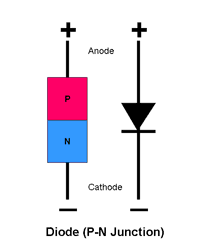
\includegraphics[height=4.2cm]{lab-02/assets/pn-diode-symbol.png}
  \caption{Symbol of a p-n junction diode \cite{lab2_polytechnichub_pn_diode}.}
  \label{fig:lab2_pn_symbol}
\end{figure}


\subsection*{Forward Bias}

In forward bias, the positive terminal of the supply is connected to the anode and the
negative terminal is connected to the cathode. The applied voltage reduces the potential
barrier across the depletion region, and once the cut-in voltage is reached the diode
current rises rapidly. For a silicon diode, the cut-in voltage is approximately
$0.7\,\text{V}$; for a germanium diode it is approximately $0.3\,\text{V}$.

For an idealized p-n junction diode, the current-voltage relationship is expressed by the
Shockley diode equation:
\[
  I_D = I_S\left(e^{V_D/(\eta V_T)} - 1\right)
\]
where $I_D$ is the diode current, $I_S$ is the reverse saturation current, $V_D$ is the
voltage across the diode, $\eta$ is the emission coefficient, and
$V_T = kT/q \approx 26\,\text{mV}$ at room temperature. For silicon diodes, $\eta$ is
commonly close to 2 in practical low-current operation \cite{lab2_razavi2013}.
The 1N4007 used in this experiment is a general-purpose silicon rectifier diode with a
high repetitive peak reverse voltage rating, which makes it suitable for low-voltage
forward and reverse-bias observation \cite{lab2_onsemi_1n4007}.

\begin{figure}[H]
  \centering
  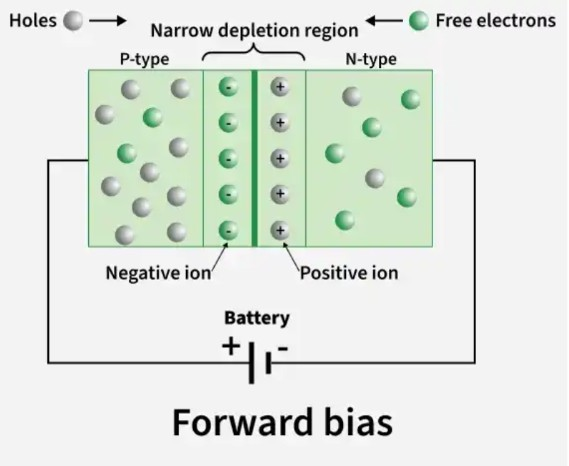
\includegraphics[width=0.88\textwidth, height=4.8cm, keepaspectratio]{lab-02/assets/forward-bias.jpg}
  \caption{Forward-bias circuit diagram used for the diode V--I study.\cite{lab2_geeksforgeeks_vi_characteristics}}
  \label{fig:lab2_forward_bias_circuit}
\end{figure}

\subsection*{Reverse Bias}

In reverse bias, the negative terminal of the supply is connected to the anode and the
positive terminal is connected to the cathode. The applied voltage widens the depletion
region and increases the potential barrier, so only a very small reverse saturation
current flows due to minority carriers.

If the reverse voltage is increased beyond the breakdown rating, avalanche or Zener
breakdown may occur. In this experiment the reverse voltage is kept low, so the diode
behaves almost like an open switch in reverse bias.

\begin{figure}[H]
  \centering
  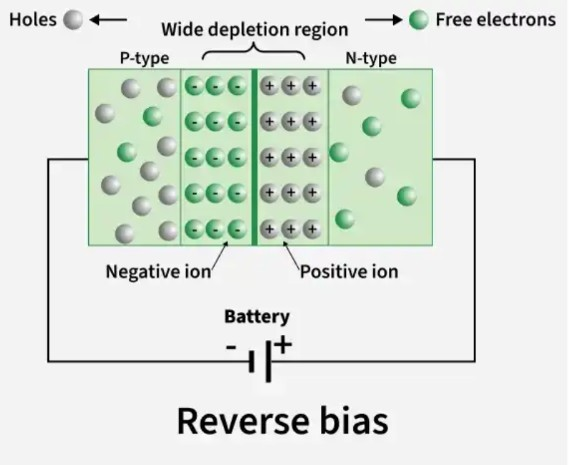
\includegraphics[width=0.88\textwidth, height=4.8cm, keepaspectratio]{lab-02/assets/reverse-bias.jpg}
  \caption{Reverse-bias circuit diagram used for the diode V--I study.\cite{lab2_geeksforgeeks_vi_characteristics}}
  \label{fig:lab2_reverse_bias_circuit}
\end{figure}


\subsection*{Expected V--I Characteristic}

The forward characteristic of a silicon diode remains almost flat until the applied diode
voltage approaches the knee region. Beyond that point, a small increase in diode voltage
produces a large increase in current, while the reverse characteristic stays nearly
horizontal because the reverse current is very small \cite{lab2_boylestad2015,lab2_onsemi_1n4007}.

\begin{figure}[H]
  \centering
  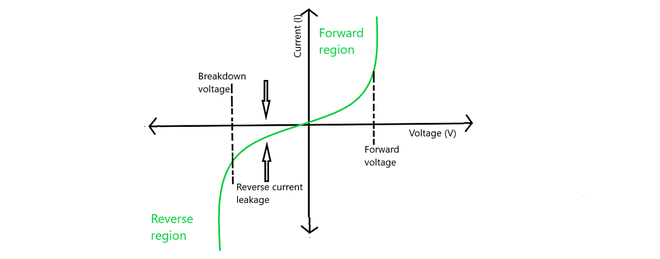
\includegraphics[width=0.88\textwidth, keepaspectratio]{lab-02/assets/vi-characteristics.png}
  \caption{V--I characteristics of p-n junction diode \cite{lab2_geeksforgeeks_vi_characteristics}.}
  \label{fig:lab2_vi_characteristics}
\end{figure}
